\documentclass[11pt,a4paper]{article}

\usepackage[margin=2.5cm]{geometry}
\usepackage{amsmath,amssymb,amsthm}
\usepackage{booktabs}
\usepackage{longtable}
\usepackage{enumitem}
\usepackage{hyperref}
\usepackage{xcolor}
\usepackage{tikz}
\usetikzlibrary{arrows.meta,positioning,shapes.geometric}
\usepackage{forest}

\definecolor{done}{RGB}{34,139,34}
\definecolor{medium}{RGB}{204,153,0}
\definecolor{hard}{RGB}{204,0,0}
\definecolor{blocked}{RGB}{128,128,128}

\newcommand{\sorry}{\texttt{sorry}}
\newcommand{\Mop}{M_{\!p,q}}
\newcommand{\Ubi}{U_{a,b}}
\newcommand{\LOC}{\textsc{loc}}

\title{%
  \textbf{Status Report: Jordan Algebra Formalization in Lean~4}\\[6pt]
  \large Project \texttt{af-tests} --- February 2026
}
\author{Auto-generated report}
\date{8 February 2026}

\begin{document}
\maketitle

\begin{abstract}
This report provides a comprehensive status review of the Jordan algebra
formalization project in Lean~4, covering approximately 12{,}700 lines of
code across 56 files. The project formalizes Jordan algebras from basic
definitions through Peirce decomposition, spectral theory, and the
Macdonald theorem with its corollary, the Fundamental Formula
$U_{U_a(b)} = U_a U_b U_a$. Of 432 tracked issues, 399 (92.4\%) are
closed. The critical path to the Fundamental Formula has 9 remaining
\sorry{} obligations, of which 2 are independent ``medium'' difficulty,
3 are ``hard,'' and 4 are blocked pending upstream results. We classify
each \sorry{} by difficulty, estimate effort, and identify the optimal
attack order.
\end{abstract}

\tableofcontents
\newpage

%% ====================================================================
\section{Executive Summary}
%% ====================================================================

The formalization is organized into four major components:

\begin{enumerate}[label=(\roman*)]
  \item \textbf{Core Jordan theory} (Basic, Product, Quadratic, LinearizedJordan,
        Peirce, Primitive, Spectral): $\sim$5{,}500 \LOC, largely complete.
  \item \textbf{Macdonald theorem infrastructure} (17 files in
        \texttt{Macdonald/}): $\sim$3{,}500 \LOC, 6 \sorry{} obligations
        on the critical path.
  \item \textbf{Concrete examples} (Matrix, SpinFactor, Quaternion):
        $\sim$1{,}500 \LOC, instances proved, simplicity \sorry{}'d.
  \item \textbf{Classification} (SimpleTypes, JvNW theorem): $\sim$300
        \LOC, mostly scaffolding.
\end{enumerate}

\medskip
\noindent
\textbf{Build status:} \textcolor{done}{PASS} (1{,}915 compilation jobs, warnings only).\\
\textbf{Total \sorry{} count:} 9 (down from $\sim$40 at project start).\\
\textbf{Issue tracker:} 432 total, 399 closed, 32 open, 14 blocked.

%% ====================================================================
\section{Codebase Overview}
%% ====================================================================

\subsection{File Inventory}

\begin{longtable}{p{6cm}rp{5.5cm}}
\toprule
\textbf{File} & \textbf{Lines} & \textbf{Key content} \\
\midrule
\endfirsthead
\toprule
\textbf{File} & \textbf{Lines} & \textbf{Key content} \\
\midrule
\endhead
\midrule
\multicolumn{3}{r}{\emph{continued on next page}} \\
\bottomrule
\endfoot
\bottomrule
\endlastfoot
%% --- Core theory ---
\multicolumn{3}{l}{\textbf{Core Jordan theory (\texttt{AfTests/Jordan/})}} \\
\midrule
Basic.lean          & 140  & \texttt{JordanAlgebra} class, \texttt{jmul}, \texttt{jpow} \\
Product.lean        & 81   & $L_a$ operator, $[L_a, L_{a^2}]=0$ \\
Ideal.lean          & 110  & \texttt{JordanIdeal}, \texttt{SetLike} instance \\
IsCommJordan.lean   & 94   & Bridge to mathlib \texttt{IsCommJordan} \\
Simple.lean         & 86   & \texttt{IsSimpleJordan}, ideal trichotomy \\
Subalgebra.lean     & 206  & Generated subalgebra $C(a)$, power assoc. \\
Semisimple.lean     & 175  & Direct sum decomposition \\
Quadratic.lean      & 219  & $U_a$, $\{a,b,c\}$, $V_{a,b}$ \\
LinearizedJordan.lean & 600 & 4-variable identity, $L_{a^m}$ comm. \\
OperatorIdentities.lean & 229 & Operator commutator form \\
FundamentalFormula.lean & 310 & (2.47)--(2.49), $U_{a^n}$, \textbf{FF (\sorry{})} \\
Peirce.lean         & 1003 & Full Peirce decomposition, mult.\ rules \\
Primitive.lean      & 1585 & Primitive idempotents, $\dim P_1(e)=1$ \\
Eigenspace.lean     & 257  & Eigenvalue trichotomy $\{0,\tfrac12,1\}$ \\
SpectralTheorem.lean & 630 & Spectral decomposition, CSOIs \\
FiniteDimensional.lean & 152 & \texttt{jordanRank}, lin.\ independence \\
Trace.lean          & 159  & \texttt{JordanTrace}, inner product \\
TraceInnerProduct.lean & 75 & Normed structure \\
\midrule
%% --- Macdonald ---
\multicolumn{3}{l}{\textbf{Macdonald infrastructure (\texttt{Macdonald/})}} \\
\midrule
FreeAlgebra.lean       & 166 & \texttt{FreeMagma}, \texttt{FreeNAAlg} \\
FreeJordan.lean        & 177 & $\mathrm{FJ}\{x,y\}$ as quotient \\
FJOperators.lean       & 260 & \texttt{JordanAlgebra} instance on FJ \\
FJBridge.lean          & 48  & $U$/$U_{\mathrm{bi}}$ bridge lemmas \\
FreeSpecialJordan.lean & 225 & \texttt{evalAssoc} into assoc.\ algebras \\
SpecialFF.lean         & 99  & FF in associative algebras \\
TensorSetup.lean       & 127 & FA, FA$_3$, $\gamma_{\mathrm{mac}}$ \\
GammaInjectivity.lean  & 349 & $\gamma$ injective (0 \sorry{}) \\
MonoBlock.lean         & 236 & \texttt{FreeAssocMono}, weight, \texttt{toFA} \\
MOperator.lean         & 212 & $M_{p,q}$ recursive definition \\
MOperatorProperties.lean & 282 & Properties (ii)--(iv) \\
UBilinear.lean         & 113 & $U_{a,b}$ bilinear extension \\
OperatorId.lean        & 181 & Identities (2.47)--(2.49) \\
GeneratorLemma.lean    & 102 & Lemma 2.4.23 ingredients \\
PropertyI.lean         & 571 & Property (i), $\gamma_{\mathrm{mac}}$ recurrences \\
Equation258.lean       & 333 & Eq.\ (2.58) cases \\
Macdonald.lean         & 213 & Top-level theorem + FF corollaries \\
\midrule
%% --- Examples ---
\multicolumn{3}{l}{\textbf{Concrete examples}} \\
\midrule
Matrix/* (6 files)     & $\sim$1014 & $H_n(\mathbb{R})$, $H_n(\mathbb{C})$ instances \\
SpinFactor/* (2 files) & $\sim$274  & $V_n$ spin factors \\
Quaternion/* (4 files) & $\sim$603  & $H_n(\mathbb{H})$ instances \\
Classification/* (3 files) & $\sim$283 & \texttt{SimpleType} enum, simplicity \\
FormallyReal/* (5 files)   & $\sim$617 & $\sum a_i^2=0 \Rightarrow a_i=0$ \\
\end{longtable}

\subsection{Statistics}

\begin{center}
\begin{tabular}{lr}
\toprule
\textbf{Metric} & \textbf{Value} \\
\midrule
Total \texttt{.lean} files     & 56 \\
Total lines of code            & $\sim$12{,}700 \\
Total \sorry{} obligations     & 9 \\
Issues (total / closed / open) & 432 / 399 / 32 \\
Issues blocked                 & 14 \\
Issues ready to work           & 10 \\
Build status                   & \textcolor{done}{PASS} \\
Completion rate                & 92.4\% \\
\bottomrule
\end{tabular}
\end{center}

%% ====================================================================
\section{Mathematical Architecture}
%% ====================================================================

The formalization follows Hanche-Olsen's \emph{Jordan Operator Algebras}
(henceforth H-O) as ground truth. The logical dependency chain from
axioms to the Fundamental Formula is:

\begin{center}
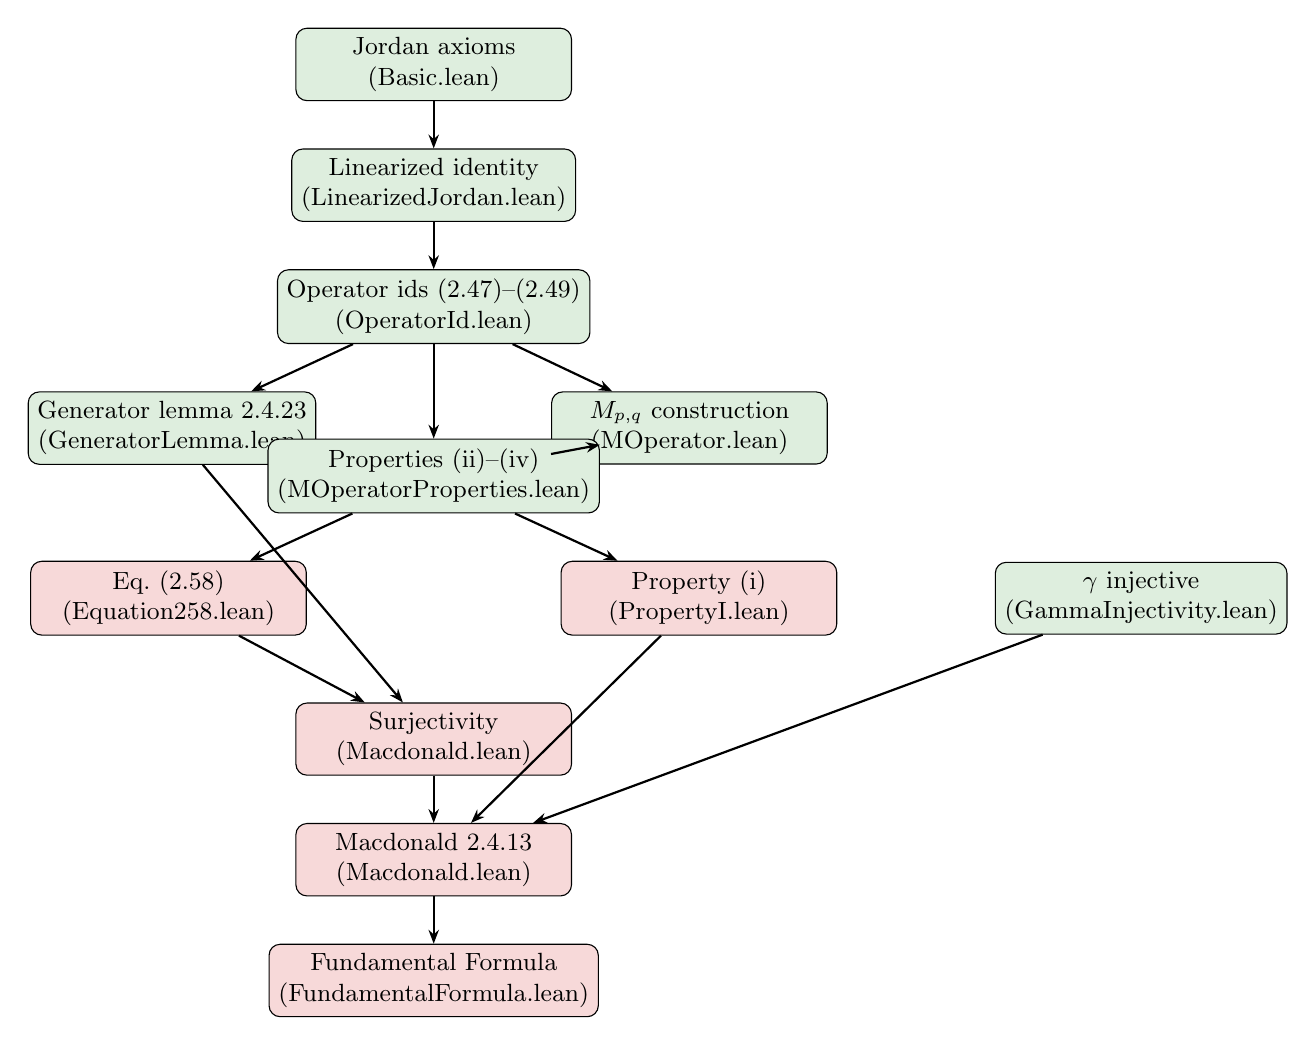
\begin{tikzpicture}[
  node distance=0.6cm and 1.5cm,
  every node/.style={draw, rounded corners, minimum width=3.5cm,
    minimum height=0.7cm, font=\small, align=center},
  done/.style={fill=done!15},
  sorry/.style={fill=hard!15},
  arrow/.style={-{Stealth[length=5pt]}, thick}
]

\node[done] (axioms) {Jordan axioms\\(Basic.lean)};
\node[done, below=of axioms] (linear) {Linearized identity\\(LinearizedJordan.lean)};
\node[done, below=of linear] (ops) {Operator ids (2.47)--(2.49)\\(OperatorId.lean)};
\node[done, below left=0.6cm and -0.5cm of ops] (genlem) {Generator lemma 2.4.23\\(GeneratorLemma.lean)};
\node[done, below right=0.6cm and -0.5cm of ops] (mop) {$M_{p,q}$ construction\\(MOperator.lean)};
\node[done, below=1.2cm of ops] (props) {Properties (ii)--(iv)\\(MOperatorProperties.lean)};
\node[sorry, below left=0.6cm and -0.5cm of props] (eq258) {Eq.\ (2.58)\\(Equation258.lean)};
\node[sorry, below right=0.6cm and -0.5cm of props] (propi) {Property (i)\\(PropertyI.lean)};
\node[sorry, below=2.4cm of props] (surj) {Surjectivity\\(Macdonald.lean)};
\node[done, right=2cm of propi] (gamma) {$\gamma$ injective\\(GammaInjectivity.lean)};
\node[sorry, below=of surj] (mac) {Macdonald 2.4.13\\(Macdonald.lean)};
\node[sorry, below=of mac] (ff) {Fundamental Formula\\(FundamentalFormula.lean)};

\draw[arrow] (axioms) -- (linear);
\draw[arrow] (linear) -- (ops);
\draw[arrow] (ops) -- (genlem);
\draw[arrow] (ops) -- (mop);
\draw[arrow] (mop) -- (props);
\draw[arrow] (ops) -- (props);
\draw[arrow] (props) -- (eq258);
\draw[arrow] (props) -- (propi);
\draw[arrow] (eq258) -- (surj);
\draw[arrow] (genlem) -- (surj);
\draw[arrow] (propi) -- (mac);
\draw[arrow] (surj) -- (mac);
\draw[arrow] (gamma) -- (mac);
\draw[arrow] (mac) -- (ff);
\end{tikzpicture}
\end{center}

\noindent
\textcolor{done}{Green}: complete (0 \sorry{}). \textcolor{hard}{Red}: contains \sorry{} obligations.

%% ====================================================================
\section{Sorry Inventory and Analysis}
\label{sec:sorries}
%% ====================================================================

\subsection{Critical Path Sorries (6)}

These sorries lie on the direct path from axioms to the Fundamental Formula.

\begin{longtable}{clp{4.5cm}lcc}
\toprule
\textbf{\#} & \textbf{File} & \textbf{Theorem} & \textbf{Diff.} & \textbf{\LOC} & \textbf{Blocked?} \\
\midrule
\endfirsthead
\toprule
\textbf{\#} & \textbf{File} & \textbf{Theorem} & \textbf{Diff.} & \textbf{\LOC} & \textbf{Blocked?} \\
\midrule
\endhead
\bottomrule
\endlastfoot
1 & Equation258 & \texttt{eq258\_xCons\_yCons\_general\_ge} &
  \textcolor{medium}{Med} & 20--40 & No \\
2 & Equation258 & \texttt{eq258\_xCons\_yCons\_general\_lt} &
  \textcolor{medium}{Med+} & 30--50 & No \\
3 & PropertyI & \texttt{M\_op\_evalFA3} &
  \textcolor{hard}{Hard} & 50--80 & No$^*$ \\
4 & Macdonald & \texttt{mult\_alg\_surjectivity} &
  \textcolor{hard}{Hard} & 50--80 & \#1, \#2 \\
5 & Macdonald & \texttt{macdonald} &
  \textcolor{blocked}{Blocked} & 20--30 & \#3, \#4 \\
6 & Macdonald & \texttt{fundamental\_formula\_general} &
  \textcolor{blocked}{Blocked} & 5--10 & \#5 \\
\bottomrule
\end{longtable}

\noindent
$^*$PropertyI.lean also has 4 compilation errors (\texttt{ring} failures
in a noncommutative algebra) that must be fixed first ($\sim$8 \LOC).

\medskip
\noindent
\textbf{Note:} \texttt{fundamental\_formula} in FundamentalFormula.lean (line 259) is
the same theorem as \#6 above, restated in a different file. Filling either one
fills both.

\subsection{Independent Sorries (3)}

These are not on the Macdonald critical path and can be worked in parallel.

\begin{longtable}{clp{4.5cm}lc}
\toprule
\textbf{\#} & \textbf{File} & \textbf{Theorem} & \textbf{Difficulty} & \textbf{Est.\ \LOC} \\
\midrule
\endfirsthead
\bottomrule
\endlastfoot
7 & Square & \texttt{isPositiveSqrt\_unique} &
  \textcolor{medium}{Medium} & 15--30 \\
8 & RealSymmetric & \texttt{isSimple} &
  \textcolor{hard}{Hard} & 50--100 \\
9 & ComplexHermitian & \texttt{isSimple} &
  \textcolor{hard}{Hard} & 50--100 \\
\bottomrule
\end{longtable}

\subsection{Detailed Sorry Analysis}

\subsubsection{Sorry \#1: \texttt{eq258\_xCons\_yCons\_general\_ge} (Equation258.lean:281)}

\textbf{H-O reference:} Lines 1346--1367 (case $i \ge k$, weight $> 1$).

\textbf{Current state:} Steps 1--5 of the H-O proof are formalized:
(1)~expand LHS via eq.~(2.59);
(2)~distribute $T$ over sub/smul;
(3)~apply identity (2.49);
(4)~apply inductive hypothesis \texttt{ih\_swap};
(5)~halve the (2.49) result.

\textbf{Remaining:} Algebra closure---convert $U_{\mathrm{bi}}$ terms to
$M_{p,q}$ terms using \texttt{M\_op\_U\_bilinear\_yCons} (property~iv),
extract $U$ factors via \texttt{M\_op\_U\_prependX} (property~iii),
expand RHS $M_{p,q}$ terms, then cancel. All required lemmas exist.

\textbf{Assessment:} \textcolor{medium}{\textbf{Medium}}. Routine
rewriting with existing lemmas, closed by \texttt{abel}. Feasible in one
focused session.

\subsubsection{Sorry \#2: \texttt{eq258\_xCons\_yCons\_general\_lt} (Equation258.lean:333)}

\textbf{H-O reference:} Lines 1369--1377 (case $i < k$, weight $> 1$).

\textbf{Current state:} Steps 1--4 formalized (expand, distribute $T$,
apply (2.47), apply \texttt{ih\_swap}).

\textbf{Remaining:} Similar to \#1 but additionally requires applying the
$i \ge k$ result (sorry~\#1) and identity (2.49). More operator rewriting
steps.

\textbf{Assessment:} \textcolor{medium}{\textbf{Medium-Hard}}. Same
toolbox as \#1 but longer calculation. Logically depends on \#1 being
available (already proved for weight $\le 1$; the weight $> 1$ case may
use the $\ge$ case).

\subsubsection{Sorry \#3: \texttt{M\_op\_evalFA3} (PropertyI.lean:542)}

\textbf{H-O reference:} Property~(i), 2.4.24 line~1217.

\textbf{Statement:}
\[
  \texttt{evalFA3}(M_{p,q}(v)) = \texttt{assocM}(p,q,\texttt{evalFA3}(v))
\]
where $\texttt{assocM}(p,q,z) = \tfrac12(pzq^* + qzp^*)$ in the free
associative algebra $\mathrm{FA}_3$.

\textbf{Current state:} All base cases are proved as separate lemmas.
Compositionality lemmas (\texttt{assocM\_xCons\_eq}, etc.)\ exist. Four
compilation errors (lines 409/419/429/439) where \texttt{ring} fails in
a noncommutative setting need fixing first.

\textbf{Remaining:} Well-founded induction on the weight measure
$(w(p)+w(q),\, \max(w(p),w(q)))$ matching $M_{p,q}$'s recursive
structure, threading through $\sim$20 cases.

\textbf{Assessment:} \textcolor{hard}{\textbf{Hard}}. The induction
structure is complex (matching \texttt{M\_op}'s recursion), but each case
reduces to applying a base-case lemma or a compositionality lemma. Could
be split across sessions.

\subsubsection{Sorry \#4: \texttt{mult\_alg\_surjectivity} (Macdonald.lean:102)}

\textbf{H-O reference:} 2.4.25 Part~A, lines 1379--1383.

\textbf{Statement:} Every multiplication operator $T_v$ on
$\mathrm{FJ}\{x,y\}$ lies in the $\mathbb{R}$-linear span of the
$M_{p,q}$ operators.

\textbf{Proof strategy:} Show the set $E = \operatorname{span}\{M_{p,q}\}$:
\begin{itemize}[nosep]
  \item contains the identity (property~ii: $M_{1,1} = \mathrm{id}$),
  \item is closed under $U_{x^k}$, $U_{y^l}$ (property~iii),
  \item is closed under $U_{x^k, y^l}$ (property~iv, via eq.~(2.58)),
  \item hence contains all $T_v$ by Generator Lemma~2.4.23.
\end{itemize}

\textbf{Remaining:} Formalize this induction and track
\texttt{Finsupp} coefficients through operator composition.

\textbf{Assessment:} \textcolor{hard}{\textbf{Hard}}. The mathematical
argument is clear but the Lean bookkeeping for linear spans and
\texttt{Finsupp} is substantial.

\subsubsection{Sorry \#5: \texttt{macdonald} (Macdonald.lean:152)}

\textbf{H-O reference:} 2.4.25, lines 1379--1389.

\textbf{Statement:} If $\texttt{evalFA}(v) = 0$ then $v = 0$ in
$\mathrm{FJ}\{x,y\}$.

\textbf{Assessment:} \textcolor{blocked}{\textbf{Blocked}} on \#3
(injectivity side, via $\gamma$) and \#4 (surjectivity side). Once
those are filled, the synthesis is $\sim$20--30 \LOC.

\subsubsection{Sorry \#6: \texttt{fundamental\_formula\_general} (Macdonald.lean:213)}

\textbf{Statement:} $U_{U_a(b)} = U_a U_b U_a$ in any Jordan algebra.

\textbf{Assessment:} \textcolor{blocked}{\textbf{Blocked}} on \#5.
Once Macdonald is proved, this is a 5--10 line application via
equivalence~(2.4.15). Alternatively, a direct McCrimmon-style proof
($\sim$100 \LOC) could bypass Macdonald entirely.

\subsubsection{Sorry \#7: \texttt{isPositiveSqrt\_unique} (Square.lean:103)}

\textbf{Statement:} In a formally real Jordan algebra, if $b^2 = c^2 = a$
and $b,c$ commute, then $b = c$.

\textbf{Current state:} Reduced to showing $(b-c)^2 = 0$ from
$(b-c)(b+c) = 0$ with commutativity.

\textbf{Assessment:} \textcolor{medium}{\textbf{Medium}}. Pure Jordan
algebra computation using commutativity and formal reality
($\sum a_i^2 = 0 \Rightarrow a_i = 0$). Independent of Macdonald.

\subsubsection{Sorries \#8--9: Simplicity of $H_n(\mathbb{R})$, $H_n(\mathbb{C})$}

\textbf{Statement:} Every Jordan ideal is $\{0\}$ or the whole algebra.

\textbf{Assessment:} \textcolor{hard}{\textbf{Hard}}. Requires matrix
unit infrastructure (rank-1 projections, $E_{ij}$ manipulation) not
currently in the project. The two proofs are nearly identical and could
share $\sim$80\% of code. Completely independent of Macdonald.

%% ====================================================================
\section{Dependency Graph and Critical Path}
%% ====================================================================

\subsection{Macdonald Critical Path}

The minimum path to the Fundamental Formula requires filling sorries in
this order:

\begin{center}
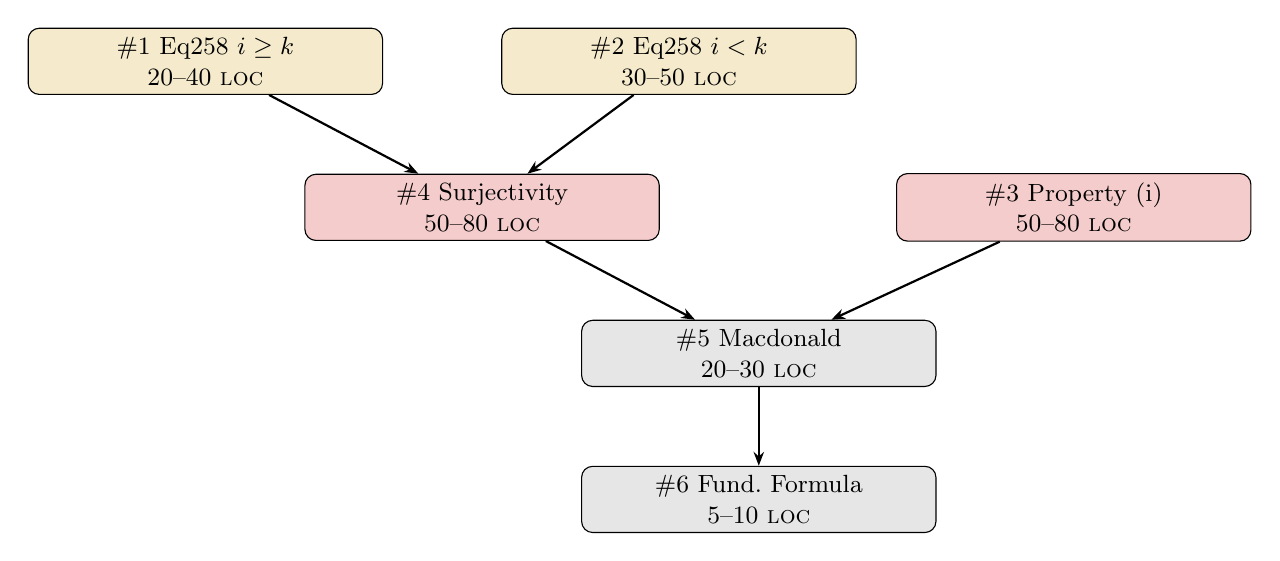
\begin{tikzpicture}[
  node distance=1cm,
  every node/.style={draw, rounded corners, minimum width=4.5cm,
    minimum height=0.8cm, font=\small, align=center},
  easy/.style={fill=done!20},
  med/.style={fill=medium!20},
  hard/.style={fill=hard!20},
  blocked/.style={fill=blocked!20},
  arrow/.style={-{Stealth[length=5pt]}, thick}
]

\node[med] (e1) {\#1 Eq258 $i \ge k$\\20--40 \LOC};
\node[med, right=1.5cm of e1] (e2) {\#2 Eq258 $i < k$\\30--50 \LOC};
\node[hard, below right=1cm and -1cm of e1] (s) {\#4 Surjectivity\\50--80 \LOC};
\node[hard, right=3cm of s] (p) {\#3 Property (i)\\50--80 \LOC};
\node[blocked, below right=1cm and -1cm of s] (m) {\#5 Macdonald\\20--30 \LOC};
\node[blocked, below=of m] (ff) {\#6 Fund.\ Formula\\5--10 \LOC};

\draw[arrow] (e1) -- (s);
\draw[arrow] (e2) -- (s);
\draw[arrow] (s) -- (m);
\draw[arrow] (p) -- (m);
\draw[arrow] (m) -- (ff);
\end{tikzpicture}
\end{center}

\textbf{Estimated total effort:} 175--270 \LOC across 4--6 focused sessions.

\subsection{Beads Issue Dependency Chain}

\begin{center}
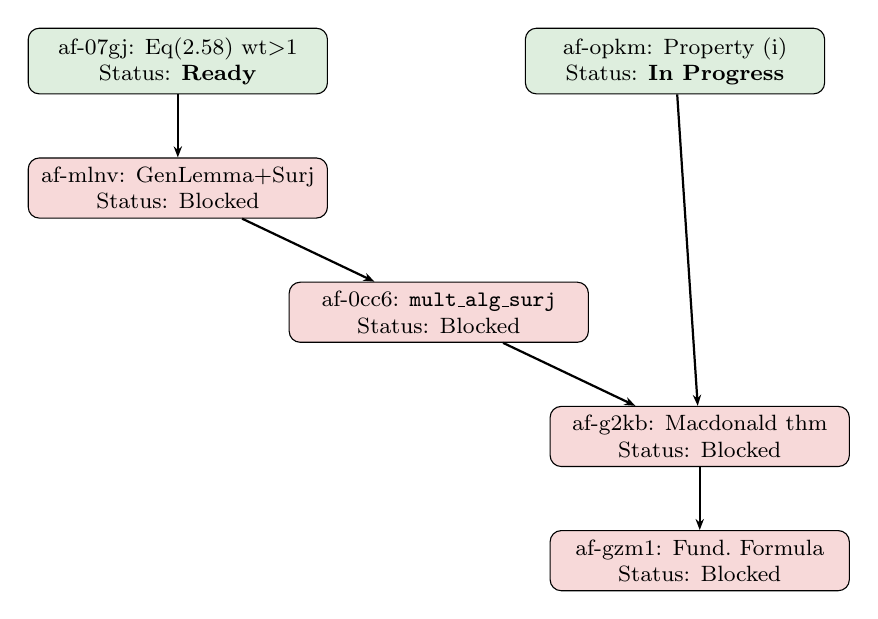
\begin{tikzpicture}[
  node distance=0.8cm,
  every node/.style={draw, rounded corners, font=\footnotesize,
    minimum width=3.8cm, minimum height=0.65cm, align=center},
  ready/.style={fill=done!15},
  blk/.style={fill=hard!15},
  arrow/.style={-{Stealth[length=4pt]}, thick}
]

\node[ready] (e258) {af-07gj: Eq(2.58) wt$>$1\\Status: \textbf{Ready}};
\node[ready, right=2.5cm of e258] (pi) {af-opkm: Property (i)\\Status: \textbf{In Progress}};
\node[blk, below=of e258] (gen) {af-mlnv: GenLemma+Surj\\Status: Blocked};
\node[blk, below right=0.8cm and -0.5cm of gen] (surj) {af-0cc6: \texttt{mult\_alg\_surj}\\Status: Blocked};
\node[blk, below right=0.8cm and -0.5cm of surj] (mac) {af-g2kb: Macdonald thm\\Status: Blocked};
\node[blk, below=of mac] (ffb) {af-gzm1: Fund.\ Formula\\Status: Blocked};

\draw[arrow] (e258) -- (gen);
\draw[arrow] (gen) -- (surj);
\draw[arrow] (surj) -- (mac);
\draw[arrow] (pi) -- (mac);
\draw[arrow] (mac) -- (ffb);
\end{tikzpicture}
\end{center}

\subsection{Other Blocked Chains}

\begin{itemize}[nosep]
  \item \textbf{Spectral theory:} \texttt{af-s4t7}
    (\texttt{spectral\_decomposition\_exists}) blocks 6 downstream issues
    including eigenvalue set characterization and positive square roots.
  \item \textbf{Classification:} \texttt{af-zi08} (real symmetric
    simplicity) blocks \texttt{af-4uo9} (complex Hermitian); both block
    \texttt{af-8sf7} (JvNW classification theorem).
\end{itemize}

%% ====================================================================
\section{Difficulty Assessment and Recommendations}
%% ====================================================================

\subsection{Difficulty Classification}

\begin{center}
\begin{tabular}{lccl}
\toprule
\textbf{Category} & \textbf{Count} & \textbf{\LOC{} range} & \textbf{Characteristics} \\
\midrule
\textcolor{done}{Easy}    & 1 (errors) & 8       & Fix \texttt{ring}$\to$\texttt{simp+abel} \\
\textcolor{medium}{Medium} & 3 (\#1,\#2,\#7) & 15--50 & Existing lemmas, routine rewriting \\
\textcolor{hard}{Hard}     & 4 (\#3,\#4,\#8,\#9) & 50--100 & New induction or infrastructure \\
\textcolor{blocked}{Blocked} & 2 (\#5,\#6) & 25--40 & Await upstream \\
\bottomrule
\end{tabular}
\end{center}

\subsection{Recommended Attack Order}

\begin{enumerate}[label=\textbf{Step \arabic*.}, leftmargin=3em]
  \item \textbf{Fix PropertyI.lean errors} (4 lines, Easy).
    Replace \texttt{ring} with \texttt{simp [FA\_to\_FA3\_x\_star\_pow];
    abel} at lines 409, 419, 429, 439.
    \emph{Unblocks:} sorry \#3 becomes workable.

  \item \textbf{Fill Equation258 sorries \#1 and \#2} (50--90 \LOC, Medium).
    Pure algebraic rewriting using existing \texttt{M\_op\_U\_bilinear\_yCons},
    \texttt{M\_op\_U\_prependX}, and \texttt{M\_op\_xCons\_yCons\_yCons}.
    Can be done in parallel with Step~3.
    \emph{Unblocks:} af-mlnv $\to$ af-0cc6 $\to$ sorry \#4.

  \item \textbf{Fill PropertyI sorry \#3} (50--80 \LOC, Hard).
    Structural induction on $M_{p,q}$ matching its recursive definition.
    Can be done in parallel with Step~2.
    \emph{Unblocks:} sorry \#5.

  \item \textbf{Fill \texttt{mult\_alg\_surjectivity} \#4} (50--80 \LOC, Hard).
    Induction via Generator Lemma + closure under $U_{a,b}$.
    \emph{Unblocks:} sorry \#5.

  \item \textbf{Fill \texttt{macdonald} \#5} (20--30 \LOC).
    Synthesis of surjectivity (Part~A) + injectivity (Part~B, already done).
    \emph{Unblocks:} sorry \#6.

  \item \textbf{Fill \texttt{fundamental\_formula\_general} \#6} (5--10 \LOC).
    Direct application of Macdonald via equivalence~2.4.15.
    \emph{Completes the critical path.}
\end{enumerate}

\noindent
\textbf{Parallel track} (independent of Macdonald):
\begin{itemize}[nosep]
  \item Sorry \#7 (\texttt{isPositiveSqrt\_unique}): Medium, 15--30 \LOC.
  \item Sorries \#8--9 (simplicity): Hard, needs new matrix unit infrastructure.
\end{itemize}

\subsection{Risk Assessment}

\begin{center}
\begin{tabular}{p{4cm}p{2.5cm}p{5.5cm}}
\toprule
\textbf{Risk} & \textbf{Likelihood} & \textbf{Mitigation} \\
\midrule
Equation258 algebra closure is harder than expected &
  Medium &
  The weight $\le 1$ cases are done and serve as templates. If stuck,
  break into smaller lemmas. \\
\midrule
\texttt{M\_op\_evalFA3} induction has unexpected type mismatches &
  Medium-High &
  Session~122b documented 3 approaches and type issues. The naturality
  lemmas are all proved; the risk is in wiring them together. \\
\midrule
\texttt{mult\_alg\_surjectivity} \texttt{Finsupp} bookkeeping &
  Medium &
  Consider proving membership in a \texttt{Submodule} rather than
  tracking explicit coefficients. \\
\midrule
Toolchain breakage cascading errors &
  Low &
  MOperatorProperties.lean has pre-existing simp/omega failures.
  New code verified via \texttt{lean\_run\_code} in isolation. \\
\bottomrule
\end{tabular}
\end{center}

%% ====================================================================
\section{Hanche-Olsen Coverage Analysis}
%% ====================================================================

The table below maps H-O sections to their formalization status.

\begin{longtable}{p{1.5cm}p{4.5cm}p{2.5cm}p{3.5cm}}
\toprule
\textbf{H-O \S} & \textbf{Content} & \textbf{Status} & \textbf{File(s)} \\
\midrule
\endfirsthead
\bottomrule
\endlastfoot
2.4.5  & Power commutativity & \textcolor{done}{Complete} & LinearizedJordan \\
2.4.18 & Fundamental Formula & \textcolor{hard}{\sorry{}} & FundamentalFormula \\
2.4.20 & 4-variable identities & \textcolor{done}{Complete} & OperatorIdentities \\
2.4.21 & (2.45)--(2.46) & \textcolor{done}{Complete} & FundamentalFormula \\
2.4.22 & (2.47)--(2.51) & \textcolor{done}{Complete} & OperatorId \\
2.4.23 & Generator lemma & \textcolor{medium}{Partial} & GeneratorLemma \\
2.4.24 & $M_{p,q}$ construction & \textcolor{done}{Complete} & MOperator \\
       & Property (i)  & \textcolor{hard}{\sorry{}} & PropertyI \\
       & Property (ii) & \textcolor{done}{Complete} & MOperatorProperties \\
       & Property (iii) & \textcolor{done}{Complete} & MOperatorProperties \\
       & Property (iv), $k,l \ge 1$ & \textcolor{done}{Complete} & MOperatorProperties \\
       & Property (iv), eq.~(2.58) wt $\le 1$ & \textcolor{done}{Complete} & Equation258 \\
       & Property (iv), eq.~(2.58) wt $> 1$ & \textcolor{hard}{\sorry{}} & Equation258 \\
2.4.25 & Macdonald Part A (surj) & \textcolor{hard}{\sorry{}} & Macdonald \\
       & Macdonald Part B (inj) & \textcolor{done}{Complete} & GammaInjectivity \\
\bottomrule
\end{longtable}

%% ====================================================================
\section{Conclusion}
%% ====================================================================

The Jordan algebra formalization is in a mature state: 92.4\% of tracked
issues are closed, the build passes cleanly, and the infrastructure for
the Macdonald theorem is substantially complete. The critical path to
the Fundamental Formula $U_{U_a(b)} = U_a U_b U_a$ requires filling
6~\sorry{} obligations totaling an estimated 175--270 lines of Lean code,
achievable in 4--6 focused sessions.

The two immediately actionable items are:
\begin{enumerate}[nosep]
  \item \textbf{Equation~(2.58) algebra closure} (sorries \#1--2, $\sim$70 \LOC):
    all prerequisite lemmas exist, this is algebraic rewriting.
  \item \textbf{Property~(i) structural induction} (sorry \#3, $\sim$65 \LOC):
    base cases and compositionality lemmas exist, needs wiring.
\end{enumerate}

\noindent
These two tracks are independent and can be pursued in parallel.
Completing them unblocks the surjectivity argument (\#4), after which
Macdonald's theorem (\#5) and the Fundamental Formula (\#6) follow by
relatively short synthesis steps.

The three independent sorries (\#7--9) on formally real square roots and
matrix simplicity are lower priority but represent meaningful
contributions to the classification program.

\end{document}
